\chapter{Architectures for written-text processing}

\section{Logistic Regression}

Before diving deeper into Neural Networks, it is useful to understand their littele brother: \textbf{Logistic Regression}. It can be used to classify an observation onto one of two classes (binary classification), or into one of many classes (multinomial classification). This section builds from the book Speech and Language Processing \cite{jurafskyspeech}.

Logistic Regression is a discriminative model, meaning that it models the conditional probability $P(y|x)$ directly, where $y$ is the class label and $x$ is the input feature vector. The model assumes a linear relationship between the input features and the log-odds of the class probabilities. A machine learning system for classification is based on four components:
\begin{enumerate}
    \item A \textbf{feature representation} of the input data, in the form of a vector of real-valued features $x = [x_1, x_2, \ldots, x_n]$;
    \item A classification function that computes $\hat{y}$, the estimated class, via $p(y|x)$ (see the \textbf{sigmoig} and \textbf{softmax} functions);
    \item An objective function for learning the model parameters from training data, minimizing error on the training set (in this case \textbf{cross-entropy loss function});
    \item An algorithm for optimizing the objective function, such as \textbf{gradient descent}.
\end{enumerate}

Starting from a single input observation $x$ represented as a vector of $n$ features $[x_1, x_2, \dots, x_n]$, the classifier output can be $1$ or $0$ in the \textbf{binary classification}. Logistic regression solves this task by learning, from a training set, a vector of \textbf{weights $W$} and a \textbf{bias term $b$} (which will be broadcasted to a vector in this case). The weight $w_i$ represents how important feature $x_i$ is to the classification decision. 
\[
z = \left(\sum_{i=1}^n w_i x_i\right) + b = \mathbf{w}^\top \mathbf{x} + b
\] 

To create a probability, then, we'll pass $z$ through the \textbf{sigmoid} function $\sigma(z)$, also called the \textbf{logistic function}. It has a domain of $(-\infty, +\infty)$ and a range of $(0, 1)$, making it suitable for modeling probabilities. 

\begin{minipage}{0.48\textwidth}
    \[
    \sigma(z) = \frac{1}{1 + e^{-z}}
    \]
\end{minipage}
\hfill
\begin{minipage}{0.48\textwidth}
    \begin{figure}[H]
    \centering
    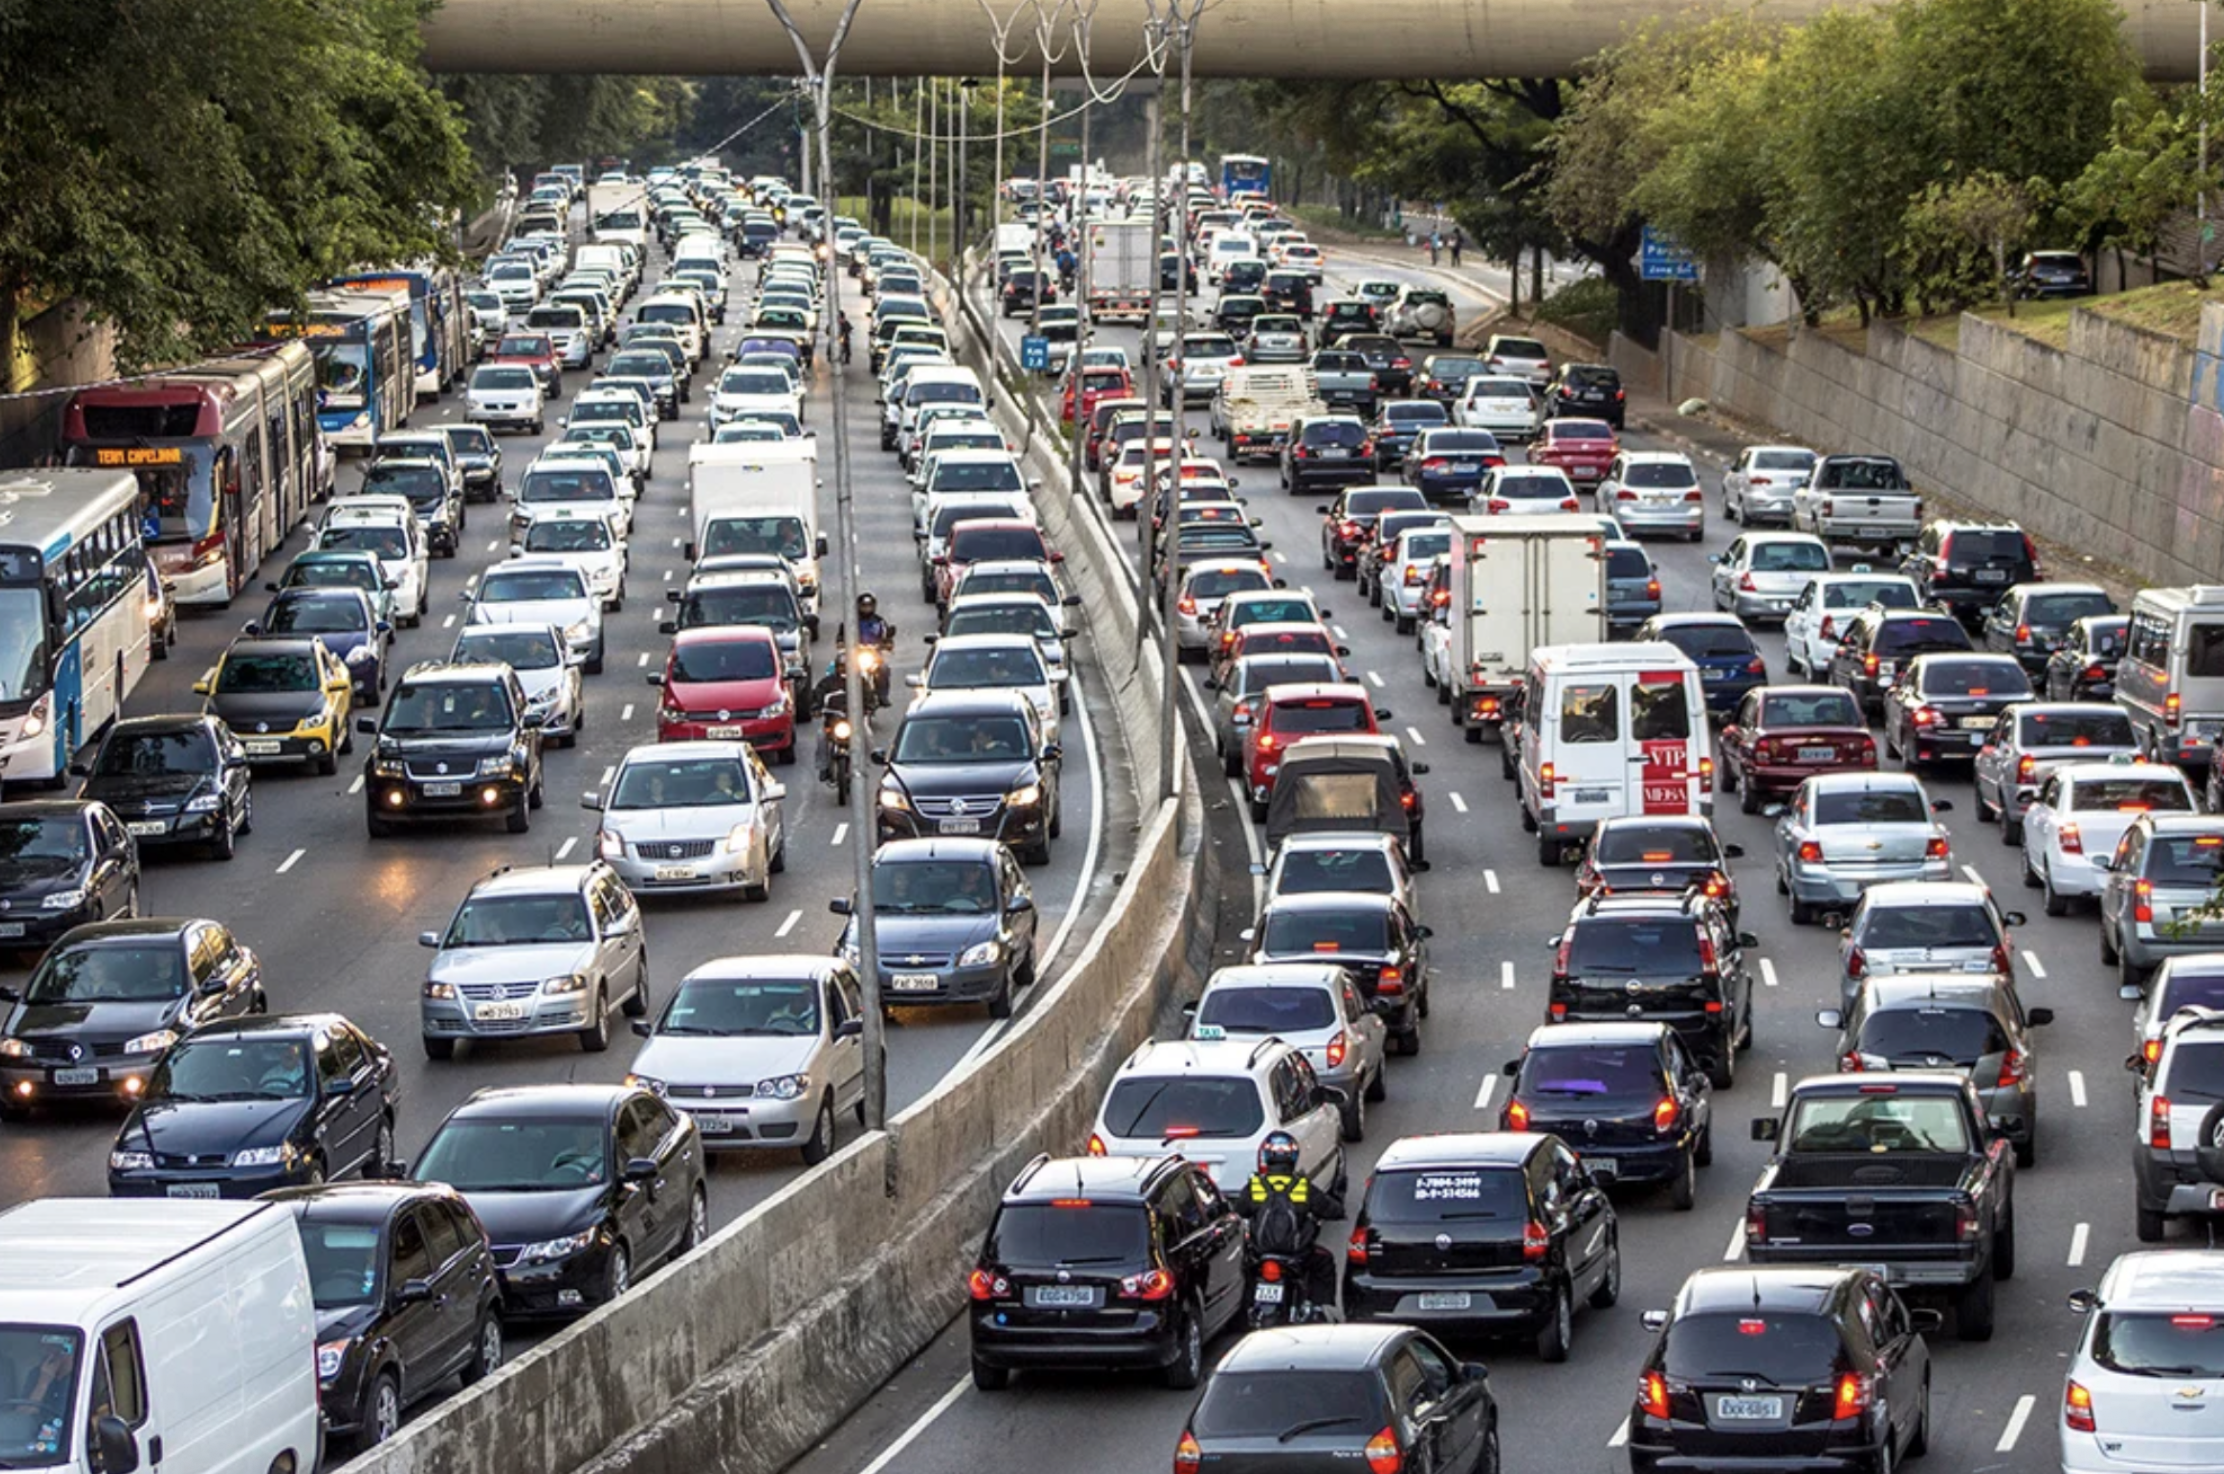
\includegraphics[width=0.6\textwidth]{assets/ch2/1.png}
\end{figure}
\end{minipage}

We can then derive the probability of class $1$ as:
\[
P(y=1|x) = \sigma(z) = \frac{1}{1 + e^{-(\mathbf{w}^\top \mathbf{x} + b)}}
\]

\begin{observationblock}
    The sigmoid function has the property
    \[
    \sigma(-z) = 1 - \sigma(z)
    \]
    which implies that
    \[
    P(y=0|x) = 1 - P(y=1|x) = \sigma(-z)
    \]
\end{observationblock}

The \textbf{decision boundary} is the value of $z$ for which we make a decision about which class to assign to a test instance $x$. Usually we set a threshold of $0.5$ for the probability of class $1$. This corresponds to $z = 0$, since $\sigma(0) = 0.5$. Therefore, if $z \geq 0$, we classify the instance as class $1$; otherwise, we classify it as class $0$.

As for now, we only consider a single example, but in practice we have to handle many of them. The most efficient approach is to use matrix multiplication to compute the outputs for all $m$ examples at once. The input data is still represented as a vector of features, but now the output must be a \textbf{one-hot vector} of $K$ values representing the classes. This way, only one of the $K$ values is $1$, indicating the correct class, while all other values are $0$. 
\[
\underbrace{\mathbf{Z}}_{(K, 1)} = \underbrace{\mathbf{W}}_{(K, n)} \underbrace{\mathbf{x}}_{(n, 1)} + \underbrace{\mathbf{b}}_{(K, 1)}
\]

Moreover, the \textbf{softmax} function is used in this case. It is a generalization of the sigmoid function for multi-class classification problems, where there are more than two classes. The softmax function takes a vector of real-valued scores (logits) and converts them into a probability distribution over multiple classes. Given a vector of logits $\mathbf{z} = [z_1, z_2, \ldots, z_k]$, the softmax function computes the probability of each class $i$ as follows:
\[
P(y=i|\mathbf{z}) = \frac{e^{z_i}}{\sum_{j=1}^k e^{z_j}}
\]

Applying the softmax function to the logistic regression model, we have to separate weight vectors $\mathbf{w}_i$ and bias $b_i$ for each of the $K$ classes. 
\[
p(y_i|\mathbf{x}) = \frac{e^{\mathbf{w}_i^\top \mathbf{x} + b_i}}{\sum_{j=1}^K e^{\mathbf{w}_j^\top \mathbf{x} + b_j}}  
\]
where $\mathbf{w}$ has shape $[n, K]$ and $\mathbf{b}$ has shape $[K, 1]$.

\[
\underbrace{\hat{y}}_{(K, 1)} = softmax(\underbrace{\mathbf{W}}_{(K, n)} \underbrace{\mathbf{x}}_{(n, 1)} + \underbrace{\mathbf{b}}_{(K, 1)})
\]

\subsection{Cross-entropy Loss Function}

We now need a loss function that expresses, for an observation $x$, how close the classifier output $\hat{y}$ is to the correct output $y$. We do this via a loss function that prefers the correct class labels of the training examples to be \textit{more likely}. We therefore choose the parameters $\mathbf{W}$ and $\mathbf{b}$ that maximize the likelihood of the correct class labels in the training data. This is equivalent to minimizing the \textbf{cross-entropy loss function}, which is defined as follows for a single training example:
\[
L(\hat{y}, y) = - \log p(y|x) = -\left[y\log\hat{y} + (1-y)\log(1-\hat{y})\right]
\]

\begin{observationblock}[Cross-entropy Loss = Negative Log-Likelihood]
    The information an event $x$ carries is defined as $I(x) = -\log P(x)$. The cross-entropy between two probability distributions $p$ and $q$ over the same set of events measures the average number of bits needed to identify an event drawn from the set, if a coding scheme used for the set is optimized for an estimated probability distribution $q$, rather than the true distribution $p$. It is defined as:
    \[
    H(p, q) = - \sum_x p(x) \log q(x)
    \]
    We can notice that the cross-entropy loss function is equivalent to the negative log-likelihood of the correct class label (look at the binary classification to understand better).
\end{observationblock}

The cross-entropy loss function can be written also as:
\[
L(\hat{y}, y) = - \sum_{i=1}^K y_i \log \hat{y}_i
\]

We now need an algorithm to minimize the loss function over the training set. A common choice is \textbf{gradient descent}, which iteratively updates the model parameters in the direction of the negative gradient of the loss function with respect to the parameters. The update rule for the weights and bias is as follows:
\[
\mathbf{W} := \mathbf{W} - \eta \nabla_{\mathbf{W}} L(\hat{y}, y)
\]
where $\eta$ is the learning rate, a hyperparameter that controls the step size of each update.

\begin{warningblock}
    To use the gradient descent algorithm, we need to be able to compute the gradient of the loss function with respect to the model parameters. This is done using the \textbf{backpropagation} algorithm, which efficiently computes the gradients by applying the chain rule of calculus, but also introduces the need to have proper differentiable functions in the model. 
\end{warningblock}

The gradient descent algorithm can be applied in two main ways: \textbf{batch gradient descent} and \textbf{stochastic gradient descent (SGD)}. In batch gradient descent, the gradients are computed using the entire training set, while in SGD, the gradients are computed using a single training example at a time. A compromise between these two approaches is \textbf{mini-batch gradient descent}, where the gradients are computed using a small subset of the training set (mini-batch) at each iteration.

It's now time to generalize the loss function from 2 to $K$ classes. We represent both $y$ and $\hat{y}$ as vectors, and the loss function is the sum of the logs of th $K$ output classes, each weighted by their probability $y_i$:

\begin{align*}
L(\hat{y}, y) &= - \sum_{i=1}^K y_i \log \hat{y}_i \\
&= - \log \hat{\mathbf{y_c}} \quad \text{(where } c \text{ is the correct class)} \\
&= -\log \frac{\exp{\mathbf{w}_c \mathbf{x} + b_c}}{\sum_{j=1}^K \exp{\mathbf{w}_j \mathbf{x} + b_j}} \\
\end{align*}

Moreover, we can derive the partial derivative of the loss with respect to $\mathbf{w}_{k,i}$ as:
\[
\frac{\partial L}{\partial \mathbf{w}_{k,i}} = (\hat{y}_i - y_i) x_k
\]

\begin{advancedblock}[Deriving the Gradient Equation]
    The \textbf{chain rule} is a fundamental rule in calculus that allows us to compute the derivative of a composite function. It states that if we have two functions $f(g(x))$, then the derivative of the composite function with respect to $x$ is given by:
    \[
    \frac{d}{dx} f(g(x)) = f'(g(x)) \cdot g'(x)
    \]
    Using the chain rule, we can derive the partial derivative of the loss function with respect to $\mathbf{w}_{k,i}$ as follows:
    \begin{align*}
    \frac{\partial L}{\partial \mathbf{w}_{k,i}} &= - \frac{\partial}{\partial \mathbf{w}_{k,i}} \log \hat{y}_c \\
    &= - \frac{1}{\hat{y}_c} \cdot \frac{\partial \hat{y}_c}{\partial \mathbf{w}_{k,i}} \\
    &= - \frac{1}{\hat{y}_c} \cdot \frac{\partial}{\partial \mathbf{w}_{k,i}} \left( \frac{e^{\mathbf{w}_c \mathbf{x} + b_c}}{\sum_{j=1}^K e^{\mathbf{w}_j \mathbf{x} + b_j}} \right) \\
    &= - \frac{1}{\hat{y}_c} \cdot \left( \frac{e^{\mathbf{w}_c \mathbf{x} + b_c} x_k (\delta_{i,c} - \hat{y}_i)}{\sum_{j=1}^K e^{\mathbf{w}_j \mathbf{x} + b_j}} \right) \\
    &= - (1) x_k (\delta_{i,c} - \hat{y}_i) \\
    &= (\hat{y}_i - y_i) x_k
    \end{align*}
    where $\delta_{i,c}$ is the Kronecker delta, which is $1$ if $i = c$ and $0$ otherwise.
\end{advancedblock}

\newpage
\section{Embeddings}

Vector semantics is the standard way to represent word meaning in NLP. It derives from two ideas: using a point in a 3D space to represent the connotation of a word and defining the meaning of a word by its \textbf{distribution} in language use, considering the neighborhood of words that tend to occur near it. 

\begin{definitionblock}[Embeddings]
    An \textbf{embedding} is simply a multidimensional vector to represent words or other discrete items. The idea is to map each word to a point in a continuous vector space, where semantically similar words are mapped to nearby points. 
\end{definitionblock}

They are \textbf{dense} vectors, meaning that the number of dimensions is much lower than the vocabulary size $|V|$, and these dimensions don't have a clear interpretation. Having dense vectors instead of sparse ones helps in different tasks, since we have to learn much less weights. Here we will dive deeper into one model: the \textbf{skip-gram with negative sampling (SGNS)}, usually referred to also as Word2Vec.

\begin{observationblock}[Cosine Similarity]
    To measure similarity between two target words $v$ and $w$, we need a metric that takes two vectors (of the same dimensionality) and gives a measure of similarity. We consider here the \textbf{cosine similarity}, which measures the angle between the two vectrs. It is based on the dot product, in fact it is a \textbf{normalized dot product}, corrected since the normal one favors long vectors ($|\mathbf{v}|$):
    \[
    cosine(\mathbf{v}, \mathbf{w}) = \frac{\mathbf{v}\cdot\mathbf{w}}{|\mathbf{v}||\mathbf{w}|} = \frac{\sum_{i=1}^N v_i w_i}{\sqrt{\sum_{i=1}^N v_i^2}\sqrt{\sum_{i=1}^N w_i^2}}
    \] 
    The cosine value ranges from 1 for vectors pointing in the same direction, through 0 for orthogolan vectors, to -1 for vectors pointing in opposite directions. 
\end{observationblock}

Word2Vec embeddings are \textbf{static embeddings}, meaning that the method learns one fixed embedding for each word in the vocaboulary, contrary to the \textbf{contextual embeddings} that will be later explained. Its intuition is to train a classifier on a binary prediction task ("Is word $w$ likely to show up near word $c$?") and then use the learned weights (initialized randomly) as embeddings. It seems like a cycle, but remember that the embeddings are the weights and the whole procedure of learning them is the algorithm. An important consideration is that we can apply \textbf{self-supervision} in this case, since we can check in an online way if our prediction is corrext just by using running text.

Given a text, we want to train a classifier such that, given a tuple $(w,c)$ of a target word $w$ paired with a candidate context word $c$, it will return the probability that $c$ is a real context word. 

\[
P(+|w,c)
\]

To compute this probability, we use embedding similarity: a word is likely to occur near the target if its embeddings (weights) are simiar to the ones of the target. We then consider the \textbf{dot product}:

\[
Similarity(w,c) \approx \mathbf{c} \cdot \mathbf{w}
\]

To have a probability, we then use the \textbf{sigmoid} function:

\[
P(+|w,c) = \sigma(\mathbf{c}\cdot\mathbf{w}) = \frac{1}{1 + e^{-\mathbf{c}\cdot\mathbf{w}}}
\]

Since we also need the total probability of all the cases to be 1, and simplifying using the independence assumption, we have that:

\[
P(+|w,c_{1:L}) = \prod_{i=1}^L P(+|w,c_i) = \prod_{i=1}^L \sigma(\mathbf{c}_i \cdot \mathbf{w})
\]

Skip-gram stores \textbf{two embeddings} for each word: the \textbf{target embedding} (used when the word is the target word $w$) and the \textbf{context embedding} (used when the word is a context word $c$). This way, we can have different representations for words depending on their role in the prediction task.

\begin{figure}[H]
    \centering
    \includegraphics[width=0.7\textwidth]{assets/ch2/2.png}
    \caption{Skip-gram architecture.}
    \label{fig:skip_gram}
\end{figure}

The learning algorithm takes as input a corpus of text and a chosen vocabulary size $N$. It randomly initializes the embeddings and then iteratively shifts them for each word to be more like the embeddings of word that occur nearby in texts, and less like the embeddings of words that do not. Since we need \textbf{negative samples}, the algorithm first determines the correct pairs and then randomly samples $k$ words from the vocabulary to create negative pairs. The loss function to minimize is then:

\begin{align*}
L_{CE} &= -\log\left[P(+|w,c_{pos})\prod_{i=1}^k P(-|w,c_{neg_i})\right] \\
&= -\left[\log P(+|w,c_{pos}) + \sum_{i=1}^k \log P(-|w,c_{neg_i})\right] \\
&= -\left[\log P(+|w,c_{pos}) + \sum_{i=1}^k \log (1 - P(+|w,c_{neg_i}))\right] \\
&= -\left[\log \sigma(\mathbf{c}_{pos} \cdot \mathbf{w}) + \sum_{i=1}^k \log \sigma(-\mathbf{c}_{neg_i} \cdot \mathbf{w})\right] 
\end{align*}

This loss function is constructed such that it:
\begin{itemize}
    \item Maximizes the similarity between the target word, context word pairs ($w,c_{pos}$) drawn from the positive examples;
    \item Minimizes the similarity between the target word, context word pairs ($w,c_{neg}$) drawn from the negative examples.
\end{itemize}

We minimize this loss function using stochastic gradient descent (SGD).

\[
\mathbf{w}^{t+1} = \mathbf{w}^t - \eta \left[\left[\sigma(\mathbf{c}_{pos}\cdot\mathbf{w}^t) - 1\right]\mathbf{c}_{pos} + \sum_{i=1}^k\left[\sigma(\mathbf{c}_{neg_i}\cdot\mathbf{w}^t)\right]\mathbf{c}_{neg_i}\right]
\]

For proofs and more details, refer to \cite{jurafskyspeech}.